\documentclass[10pt,a4paper]{article}
\usepackage[UTF8,fontset = windows]{ctex}
\setCJKmainfont[BoldFont=黑体,ItalicFont=楷体]{华文中宋}
\usepackage{amssymb,amsmath,amsfonts,amsthm,mathrsfs,dsfont,graphicx}
\usepackage{ifthen,indentfirst,enumerate,color,titletoc}
\usepackage{tikz}
\usepackage{multicol}
\usepackage{makecell}
\usepackage{longtable}
\usetikzlibrary{arrows,calc,intersections,patterns,decorations.pathreplacing,3d,angles,quotes,positioning}
\usepackage[bf,small,indentafter,pagestyles]{titlesec}
\usepackage[top=1in, bottom=1in,left=0.8in,right=0.8in]{geometry}
\renewcommand{\baselinestretch}{1.65}
\newtheorem{defi}{定义~}
\newtheorem{eg}{例~}
\newtheorem{ex}{~}
\newtheorem{rem}{注~}
\newtheorem{thm}{定理~}
\newtheorem{coro}{推论~}
\newtheorem{axiom}{公理~}
\newtheorem{prop}{性质~}
\newcommand{\blank}[1]{\underline{\hbox to #1pt{}}}
\newcommand{\bracket}[1]{(\hbox to #1pt{})}
\newcommand{\onech}[4]{\par\begin{tabular}{p{.9\textwidth}}
A.~#1\\
B.~#2\\
C.~#3\\
D.~#4
\end{tabular}}
\newcommand{\twoch}[4]{\par\begin{tabular}{p{.46\textwidth}p{.46\textwidth}}
A.~#1& B.~#2\\
C.~#3& D.~#4
\end{tabular}}
\newcommand{\vartwoch}[4]{\par\begin{tabular}{p{.46\textwidth}p{.46\textwidth}}
(1)~#1& (2)~#2\\
(3)~#3& (4)~#4
\end{tabular}}
\newcommand{\fourch}[4]{\par\begin{tabular}{p{.23\textwidth}p{.23\textwidth}p{.23\textwidth}p{.23\textwidth}}
A.~#1 &B.~#2& C.~#3& D.~#4
\end{tabular}}
\newcommand{\varfourch}[4]{\par\begin{tabular}{p{.23\textwidth}p{.23\textwidth}p{.23\textwidth}p{.23\textwidth}}
(1)~#1 &(2)~#2& (3)~#3& (4)~#4
\end{tabular}}
\begin{document}

\begin{enumerate}[1.]

\item { (002716)}已知集合$M=\{x|x=3m+1, \ m\in \mathbf{Z}\}$, $N=\{y|y=3m+2, \ m\in \mathbf{Z}\}$, 若$x_0\in M$, $y_0\in N$, 则$x_0y_0$与集合$M,N$的关系是\bracket{20}.
\twoch{$x_0y_0\in M$但$x_0y_0$$\notin N$}{$x_0y_0\in N$但$x_0y_0\notin M$}{$x_0y_0\notin M$且$x_0y_0\notin N$}{$x_0y_0$$\in M$且$x_0y_0\in N$}


关联目标:

暂未关联目标



标签: 第一单元

答案: 暂无答案

解答或提示: 暂无解答与提示

使用记录:

暂无使用记录


出处: 2022届高三第一轮复习讲义
\item { (004781)}已知集合$A=\{x|\dfrac{12}{5-x}\in \mathbf{N},\ x\in\mathbf{Z}\}$, 用列举法表示集合$A$.


关联目标:

暂未关联目标



标签: 暂无标签

答案: 暂无答案

解答或提示: 暂无解答与提示

使用记录:

暂无使用记录


出处: 代数精编第一章集合与命题
\item { (004794)}已知非空集合$P$满足: \textcircled{1} $P\subseteq \{1,2,3,4,5\}$; \textcircled{2} 若$a\in P$, 则$6-a\in P$. 符合上述要求的集合P的个数是\bracket{20}.
\fourch{$4$}{$5$}{$7$}{$31$}


关联目标:

暂未关联目标



标签: 暂无标签

答案: 暂无答案

解答或提示: 暂无解答与提示

使用记录:

暂无使用记录


出处: 代数精编第一章集合与命题
\item { (004770)}已知集合$A=\{x|x^2-5x+4\le 0\}$与$B=\{x|x^2-2ax+a+2\le 0,\ a\in \mathbf{R}\}$满足$B\subseteq A$, 求$a$的取值范围.


关联目标:

暂未关联目标



标签: 暂无标签

答案: 暂无答案

解答或提示: 暂无解答与提示

使用记录:

暂无使用记录


出处: 代数精编第一章集合与命题
\item { (003501)}用``$\subseteq$''连接集合$\mathbf{Z}$、$\mathbf{Q}$、$\mathbf{R}$、$\mathbf{C}$:\blank{50}.


关联目标:

暂未关联目标



标签: 第五单元

答案: 暂无答案

解答或提示: 暂无解答与提示

使用记录:

暂无使用记录


出处: 2022届高三第一轮复习讲义
\item { (002693)}已知$P=\{y=x^2+1\}$, $Q=\{y|y=x^2+1, \ x\in \mathbf{R}\}$, $E=\{x|y=x^2+1, \  x\in \mathbf{R}\}$, $F=\{(x,y)|y=x^2+1, \ x\in \mathbf{R}\}$, $G=\{x|x\ge 1\}$, $H=\{x|x^2+1=0, \ x\in \mathbf{R}\}$, 则各集合间关系正确的有\blank{50}. (答案可能不唯一)\\
(A) $P=F$   (B) $Q=E$   (C) $E=F$   (D) $Q\subseteq G$  (E) $H\subsetneqq P$


关联目标:

暂未关联目标



标签: 第一单元

答案: 暂无答案

解答或提示: 暂无解答与提示

使用记录:

暂无使用记录


出处: 2022届高三第一轮复习讲义
\item { (002728)}设含有三个实数的集合既可以表示为$\{a,\dfrac ba,1\}$, 又可以表示为$\{a^2,a+b,0\}$, 那么$a+b=$\blank{50}.


关联目标:

暂未关联目标



标签: 第一单元

答案: 暂无答案

解答或提示: 暂无解答与提示

使用记录:

暂无使用记录


出处: 2022届高三第一轮复习讲义
\item { (004781)}已知集合$A=\{x|\dfrac{12}{5-x}\in \mathbf{N},\ x\in\mathbf{Z}\}$, 用列举法表示集合$A$.


关联目标:

暂未关联目标



标签: 暂无标签

答案: 暂无答案

解答或提示: 暂无解答与提示

使用记录:

暂无使用记录


出处: 代数精编第一章集合与命题
\item { (002714)}若集合$M=[a-1,a+1]$, $N=(-\infty,-1)\cup [2,+\infty)$, 且$M\cap N=\varnothing$, 则实数$a$的取值范围为\blank{50}.


关联目标:

暂未关联目标



标签: 第一单元

答案: 暂无答案

解答或提示: 暂无解答与提示

使用记录:

暂无使用记录


出处: 2022届高三第一轮复习讲义
\item { (002704)}(1) 已知集合$A=\{y|y=x^2, \ x\in \mathbf{R}\}, B=\{y|y=4-x^2, \ x\in \mathbf{R}\}$, 则$A\cap B=$\blank{50}.\\
(2) 已知集合$A=\{(x,y)|y={x^2},\ x\in \mathbf{R}\}$, $B=\{(x,y)|y=4-x^2, \ x\in \mathbf{R}\}$, 则$A\cap B=$\blank{50}.


关联目标:

暂未关联目标



标签: 第一单元

答案: 暂无答案

解答或提示: 暂无解答与提示

使用记录:

暂无使用记录


出处: 2022届高三第一轮复习讲义
\item { (007684)}用适当的方法表示下列集合:\\
(1) 方程$x^2-2=0$的实数解组成的集合;\\
(2) 两直线$y=2x+1$和$y=x-2$的交点组成的集合.


关联目标:

暂未关联目标



标签: 第一单元

答案: 暂无答案

解答或提示: 暂无解答与提示

使用记录:

暂无使用记录


出处: 二期课改练习册高一第一学期
\item { (002702)}若集合$A=[2,3]$, 集合$B=[a,2a+1]$.\\
(1) 若$A\subsetneqq B$, 求实数$a$的取值范围;\\
(2) 若$A\cap B\ne \varnothing$, 求实数$a$的取值范围.


关联目标:

暂未关联目标



标签: 第一单元

答案: 暂无答案

解答或提示: 暂无解答与提示

使用记录:

暂无使用记录


出处: 2022届高三第一轮复习讲义
\item { (002693)}已知$P=\{y=x^2+1\}$, $Q=\{y|y=x^2+1, \ x\in \mathbf{R}\}$, $E=\{x|y=x^2+1, \  x\in \mathbf{R}\}$, $F=\{(x,y)|y=x^2+1, \ x\in \mathbf{R}\}$, $G=\{x|x\ge 1\}$, $H=\{x|x^2+1=0, \ x\in \mathbf{R}\}$, 则各集合间关系正确的有\blank{50}. (答案可能不唯一)\\
(A) $P=F$   (B) $Q=E$   (C) $E=F$   (D) $Q\subseteq G$  (E) $H\subsetneqq P$


关联目标:

暂未关联目标



标签: 第一单元

答案: 暂无答案

解答或提示: 暂无解答与提示

使用记录:

暂无使用记录


出处: 2022届高三第一轮复习讲义
\item { (004768)}已知集合$U =\{x|x\text{取不大于}30\text{的质数}\}$, $A$, $B$是$U$的两个子集, 且满足$A\cap \complement_UB=\{5,13,23\}$, $\complement_A\cap B=\{11,19,29\}$, $\complement_UA\cap \complement_UB=\{3,7\}$, 求$A$, $B$.


关联目标:

暂未关联目标



标签: 暂无标签

答案: 暂无答案

解答或提示: 暂无解答与提示

使用记录:

暂无使用记录


出处: 代数精编第一章集合与命题
\item { (002700)}集合$C=\{x|x=\dfrac k2\pm \dfrac14, \ k\in \mathbf{Z}\},D=\{x|x=\dfrac k4,\ k\in \mathbf{Z}\}$, 试判断$C$与$D$的关系, 并证明.


关联目标:

暂未关联目标



标签: 第一单元

答案: 暂无答案

解答或提示: 暂无解答与提示

使用记录:

暂无使用记录


出处: 2022届高三第一轮复习讲义
\item { (002702)}若集合$A=[2,3]$, 集合$B=[a,2a+1]$.\\
(1) 若$A\subsetneqq B$, 求实数$a$的取值范围;\\
(2) 若$A\cap B\ne \varnothing$, 求实数$a$的取值范围.


关联目标:

暂未关联目标



标签: 第一单元

答案: 暂无答案

解答或提示: 暂无解答与提示

使用记录:

暂无使用记录


出处: 2022届高三第一轮复习讲义
\item { (001014)}已知集合$M=\{y|y=x+1, \ x \in \mathbf{R}\}$, $N=\{y|y=-x^2+4x,\  x \in \mathbf{R}\}$,
则$M \cap N=$\blank{80}.


关联目标:

暂未关联目标



标签: 第一单元

答案: 暂无答案

解答或提示: 暂无解答与提示

使用记录:

2016届11班	\fcolorbox[rgb]{0,0,0}{0.820,1.000,0}{0.410}

2016届12班	\fcolorbox[rgb]{0,0,0}{0.616,1.000,0}{0.308}


出处: 2016届创新班作业	1106-集合的运算
\item { (001015)}已知集合$A=\{x|\ x^2+px+q=0\}$, $B=\{x|\ x^2-x+r=0\}$, 且$A\cap B=\{-1\}$, $A\cup B=\{-1,2\}$, 求实数$p,q,r$的值.


关联目标:

暂未关联目标



标签: 第一单元

答案: 暂无答案

解答或提示: 暂无解答与提示

使用记录:

2016届11班	\fcolorbox[rgb]{0,0,0}{1.000,0.666,0}{0.667}

2016届12班	\fcolorbox[rgb]{0,0,0}{1.000,0.820,0}{0.590}


出处: 2016届创新班作业	1106-集合的运算
\item { (001016)}已知集合$A=\{1,2\}$, $B=\{x|mx^2+2mx-1<0, x \in\mathbf{R}\}$. 已知$A \cap B=\{1\}$, 求实数$m$的取值范围.


关联目标:

暂未关联目标



标签: 第一单元

答案: 暂无答案

解答或提示: 暂无解答与提示

使用记录:

2016届11班	\fcolorbox[rgb]{0,0,0}{1.000,0.410,0}{0.795}

2016届12班	\fcolorbox[rgb]{0,0,0}{1.000,0.616,0}{0.692}


出处: 2016届创新班作业	1106-集合的运算
\item { (002703)}设全集$U=\mathbf{R}$, 集合$A=\{x|f(x)=0\}$, $B=\{x|g(x)=0\}$, $C=\{x|h(x)=0, \ x\in \mathbf{R}\}$, 则方程$\dfrac{f^2(x)+g^2(x)}{h(x)}=0$的解集是\blank{50}(用$U,A,B,C$表示).


关联目标:

暂未关联目标



标签: 第一单元

答案: 暂无答案

解答或提示: 暂无解答与提示

使用记录:

暂无使用记录


出处: 2022届高三第一轮复习讲义
\item { (004769)}已知集合$A=\{x|x^2- ax+a^2-19=0\}$, $B=\{x|x^2-5x+6=0\}$, $C=\{ x|x^2+2x-8=0\}$满足$A\cap B\ne \varnothing$, $A\cap C=\varnothing$, 求实数$a$的值.


关联目标:

暂未关联目标



标签: 暂无标签

答案: 暂无答案

解答或提示: 暂无解答与提示

使用记录:

暂无使用记录


出处: 代数精编第一章集合与命题
\item { (002710)}如图, $U$为全集, $M,P,S$是$U$的三个子集, 则阴影部分所表示的集合是\bracket{20}.
\fourch{$(M\cap P)\cap S$}{$(M\cap P)\cup S$}{$(M\cap P)\cap \complement_U S$}{$(M\cap P)\cup \complement_U S$}
\begin{center}
    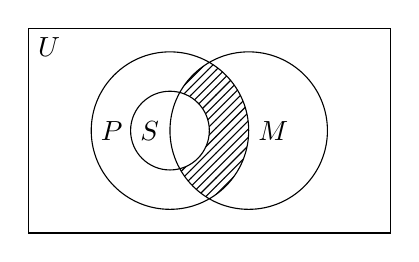
\begin{tikzpicture}
        \begin{scope}
            \clip (1,0) circle (1);
            \begin{scope}[even odd rule]
                \clip (0,0) circle (1) (0,0) circle (0.5);
                \filldraw [pattern = {north east lines}] (-2,-2) rectangle (2,2);
            \end{scope}
        \end{scope}
        \draw (0,0) circle (1) (1,0) circle (1) (0,0) circle (0.5);
        \draw (-1.8,-1.3) rectangle (2.8,1.3);
        \draw (-1.8,1.3) node [below right] {$U$} (-1,0) node [right] {$P$} (-0.5,0) node [right] {$S$} (1,0) node [right] {$M$};
    \end{tikzpicture}
\end{center}


关联目标:

暂未关联目标



标签: 第一单元

答案: 暂无答案

解答或提示: 暂无解答与提示

使用记录:

暂无使用记录


出处: 2022届高三第一轮复习讲义
\item { (002712)}设集合$A\cap \{-2,0,1\}=\{0,1\}$, $A\cup \{-2,0,2\}=\{-2,0,1,2\}$, 则满足上述条件的集合$A$的个数为\blank{50}个.


关联目标:

暂未关联目标



标签: 第一单元

答案: 暂无答案

解答或提示: 暂无解答与提示

使用记录:

暂无使用记录


出处: 2022届高三第一轮复习讲义
\item { (001015)}已知集合$A=\{x|\ x^2+px+q=0\}$, $B=\{x|\ x^2-x+r=0\}$, 且$A\cap B=\{-1\}$, $A\cup B=\{-1,2\}$, 求实数$p,q,r$的值.


关联目标:

暂未关联目标



标签: 第一单元

答案: 暂无答案

解答或提示: 暂无解答与提示

使用记录:

2016届11班	\fcolorbox[rgb]{0,0,0}{1.000,0.666,0}{0.667}

2016届12班	\fcolorbox[rgb]{0,0,0}{1.000,0.820,0}{0.590}


出处: 2016届创新班作业	1106-集合的运算
\item { (004769)}已知集合$A=\{x|x^2- ax+a^2-19=0\}$, $B=\{x|x^2-5x+6=0\}$, $C=\{ x|x^2+2x-8=0\}$满足$A\cap B\ne \varnothing$, $A\cap C=\varnothing$, 求实数$a$的值.


关联目标:

暂未关联目标



标签: 暂无标签

答案: 暂无答案

解答或提示: 暂无解答与提示

使用记录:

暂无使用记录


出处: 代数精编第一章集合与命题
\item { (002710)}如图, $U$为全集, $M,P,S$是$U$的三个子集, 则阴影部分所表示的集合是\bracket{20}.
\fourch{$(M\cap P)\cap S$}{$(M\cap P)\cup S$}{$(M\cap P)\cap \complement_U S$}{$(M\cap P)\cup \complement_U S$}
\begin{center}
    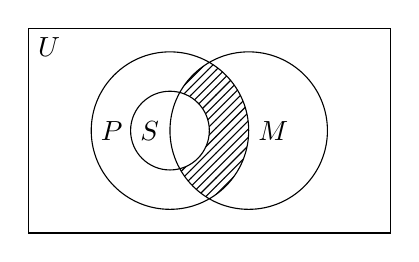
\begin{tikzpicture}
        \begin{scope}
            \clip (1,0) circle (1);
            \begin{scope}[even odd rule]
                \clip (0,0) circle (1) (0,0) circle (0.5);
                \filldraw [pattern = {north east lines}] (-2,-2) rectangle (2,2);
            \end{scope}
        \end{scope}
        \draw (0,0) circle (1) (1,0) circle (1) (0,0) circle (0.5);
        \draw (-1.8,-1.3) rectangle (2.8,1.3);
        \draw (-1.8,1.3) node [below right] {$U$} (-1,0) node [right] {$P$} (-0.5,0) node [right] {$S$} (1,0) node [right] {$M$};
    \end{tikzpicture}
\end{center}


关联目标:

暂未关联目标



标签: 第一单元

答案: 暂无答案

解答或提示: 暂无解答与提示

使用记录:

暂无使用记录


出处: 2022届高三第一轮复习讲义
\item { (002712)}设集合$A\cap \{-2,0,1\}=\{0,1\}$, $A\cup \{-2,0,2\}=\{-2,0,1,2\}$, 则满足上述条件的集合$A$的个数为\blank{50}个.


关联目标:

暂未关联目标



标签: 第一单元

答案: 暂无答案

解答或提示: 暂无解答与提示

使用记录:

暂无使用记录


出处: 2022届高三第一轮复习讲义
\item { (002697)}设全集$U=\{2,3,a^2+2a-3\}$, 集合$A=\{|2a-1|,2\}$, $\complement_U A=\{5\}$, 则实数$a=$\blank{50}.


关联目标:

暂未关联目标



标签: 第一单元

答案: 暂无答案

解答或提示: 暂无解答与提示

使用记录:

暂无使用记录


出处: 2022届高三第一轮复习讲义
\item { (002710)}如图, $U$为全集, $M,P,S$是$U$的三个子集, 则阴影部分所表示的集合是\bracket{20}.
\fourch{$(M\cap P)\cap S$}{$(M\cap P)\cup S$}{$(M\cap P)\cap \complement_U S$}{$(M\cap P)\cup \complement_U S$}
\begin{center}
    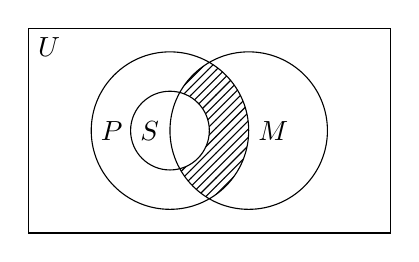
\begin{tikzpicture}
        \begin{scope}
            \clip (1,0) circle (1);
            \begin{scope}[even odd rule]
                \clip (0,0) circle (1) (0,0) circle (0.5);
                \filldraw [pattern = {north east lines}] (-2,-2) rectangle (2,2);
            \end{scope}
        \end{scope}
        \draw (0,0) circle (1) (1,0) circle (1) (0,0) circle (0.5);
        \draw (-1.8,-1.3) rectangle (2.8,1.3);
        \draw (-1.8,1.3) node [below right] {$U$} (-1,0) node [right] {$P$} (-0.5,0) node [right] {$S$} (1,0) node [right] {$M$};
    \end{tikzpicture}
\end{center}


关联目标:

暂未关联目标



标签: 第一单元

答案: 暂无答案

解答或提示: 暂无解答与提示

使用记录:

暂无使用记录


出处: 2022届高三第一轮复习讲义
\item { (002703)}设全集$U=\mathbf{R}$, 集合$A=\{x|f(x)=0\}$, $B=\{x|g(x)=0\}$, $C=\{x|h(x)=0, \ x\in \mathbf{R}\}$, 则方程$\dfrac{f^2(x)+g^2(x)}{h(x)}=0$的解集是\blank{50}(用$U,A,B,C$表示).


关联目标:

暂未关联目标



标签: 第一单元

答案: 暂无答案

解答或提示: 暂无解答与提示

使用记录:

暂无使用记录


出处: 2022届高三第一轮复习讲义
\end{enumerate}



\end{document}